\chapter{Introduction}
\label{chp:introduction}

While consumer-grade genotyping - such as that used by 23andMe - has proven a popular and inexpensive method to determine Single Nucleotide Polymorphisms (SNPs) in individuals, such methods can only detect a set of reference genes, thus limiting their ability to detect all but the simplest variations.

Whole genome sequencing (without a reference) is a powerful alternative, albeit comparatively expensive. However, the price has been steadily declining: while the Human Genome Project cost \$2.7 billion to complete in 2003~\cite{HGP}, as of 2019 it is possible to have a genome sequenced for \$299~\cite{dantelabscost}, and the price continues to drop.

This decline in price is in large part owed to the advent of Next Generation Sequencing (NGS) machines. The “Sanger” sequencing method used in the Human Genome project required a high degree of human interaction, which NGS machines have subsequently automated, greatly increasing the speed and decreasing the cost. And although NGS machines produce much shorter reads (200 bases versus 800 bases in Sanger sequencing - a human genome is 3.4 billion bases), this is overcome by re-sequencing the same DNA.

%There has been another family of DNA sequencers appearing over the past eight years, which can read an entire chromosome at a time. However, they have unpredictable error profiles, making it difficult to sanitize the data, and it is unlikely this will improve without a major breakthrough in physics (cite). Consequently, instead of replacing NGS machines, they are often used in tandem by providing a reference when combining the short read data that NGS machines produce (cite).

The process of combining short reads into longer sequences is called assembly, and while finding the best overlap is NP-hard~\cite{Mye95}, many practical approaches have been proposed (see surveys \cite{KasMor06, MilKor10, Pop09}).

Traditionally, assembly employed an overlap graph, where each read is a node, and an edge exists if two reads have sufficient overlap~\cite{BatJaf02,HuaYan05,MyeSut00}. Assembly then involves computing a Hamiltonian tour of all nodes. This was an acceptable drawback when dealing with Sanger reads, but is prohibitively expensive to deal with the abundant data that NGS machines produce.

% TODO: Do large k diagram, and single edge diagram

%\begin{figure}
%	\begin{center}
%		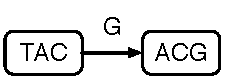
\includegraphics[scale=0.7]{images/dbg-edge.pdf}
%		\caption{An edge representing the sequence `TACG' for the $k=3$ de Bruijn graph.}
%		\label{figure:edge}
%	\end{center}
%\end{figure}

\begin{figure}
	\begin{center}
		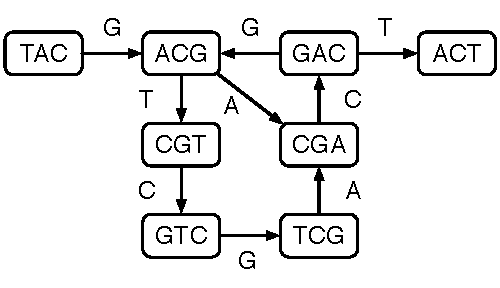
\includegraphics[scale=0.8]{images/dbg.pdf}
		\caption{The $k=3$ de Bruijn graph of reads `TACGT', `TACGA', `ACGTC', `GTCGA', `CGACT', and
			`CGACG'. The edges are given by the substrings of length $k+1=4$ from all of the reads (`TACG', `ACGA', `ACGT', `CGTC', and so on), and are represented by their right-most symbol connecting the two vertices  given by their two substrings of length $k=3$ (e.g. $TAC \xrightarrow{G} ACG$). The longest contig is found by starting at `ACG`, and following its branch labeled `T`, and all subsequent edges, until we reach another branch at vertex `GAC' (which has two edges labeled `G' and `T'), giving us `ACGTCGAC' ($8$ bases).}
		\label{figure:dbg}
	\end{center}
\end{figure}

\begin{figure}[!h]
	\begin{center}
		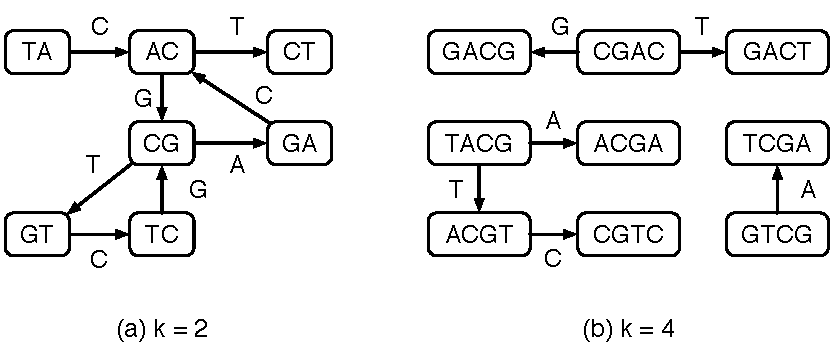
\includegraphics[scale=0.8]{images/altering-k.pdf}
		\caption{$(a)$ The $k=2$ de Bruijn graph of strings `TACGT', `TACGA', `ACGTC', `GTCGA', `CGACT', and
			`CGACG', and $(b)$ the $k=4$ de Bruijn graph of strings `TACGT', `TACGA', `ACGTC', `GTCGA', `CGACT', and
			`CGACG'. The longest contig for $(a)$ is `CGTCG' ($5$ bases), and the longest contig for $(b)$ is `TACGTC' ($6$ bases).}
		\label{figure:varying-k}
	\end{center}
\end{figure}


% TODO: take some more time to explain this
Eulerian assembly replaces the overlap graph with a de Bruijn graph~\cite{IW95, PTW}, where every $k$-length substring of the reads is a node, and the directed edges are defined by the $k+1$-length substrings that contain the $k$-length vertices, where $k$ is a user-selected parameter. For example, for $k=3$, the sequence `TACGT' yields the edges `TACG' and `ACGT', and the edge `TACG' connects the vertices `TAC' and `ACG' by dropping the initial `T' and appending a `G'. A complete example is given in Figure \ref{figure:dbg}.

\emph{Contigs} (contiguous sequences) are then found by following the edges between two branches (see Figure \ref{figure:dbg}). Most modern assembler programs use this paradigm~\cite{bankevich2012spades,peng2010idba,Li:2010,Simpson:2009,Butler:2008,SahShi12,MacPrz09,ZerBir08}. See \cite{compeau11} for a thorough explanation of de Bruijn graphs and their use in assembly.

While the de Bruijn graph can be constructed more efficiently than the overlap graph, it remains a bottleneck in assembly, both in terms of speed and size, with a de Bruijn graph of a human genome requiring 300 GB of RAM~\cite{Simpson:2009}. Previous work has reduced this to 30 GB~\cite{conway}. This thesis reduces this to 2 GB, bringing it in line with commodity hardware - a student or field biologist could now perform this on their laptop. Around the same time as the work done in this thesis, an alternative approach with similar performance was published~\cite{wabi}, but the Burrows-Wheeler based approach taken in this thesis offers more flexibility and faster edge traversal.



% TODO: Take more time to explain this
It is common for modern assemblers to build multiple de Bruijn graphs. This is because the $k$ parameter significantly influences the topology - if $k$ is too large there may be too few edges, causing gaps in the graph. But if $k$ is too small, the vertices may have too many edges, increasing ambiguity. Both of these issues lead to shorter contigs, as is demonstrated in Figure \ref{figure:varying-k}. In fact, due to non-uniform coverage of NGS data, different areas of the same graph may benefit from differing $k$ values. To overcome this, assemblers such as Spades and IDBA~\cite{bankevich2012spades,peng2010idba} build de Bruijn graphs for increasing values of $k$, and use them in tandem. This yields better quality assemblies, but is slowed down proportionally to the number of $k$ values used. This thesis introduces the first variation of the de Bruijn graph that can be built once, yet change $k$ values on-the-fly, at only a modest increase in size over the base succinct de Bruijn graph, taking only $3.5$ times the space, and only $30\%$ longer to construct than a graph for a \emph{single} value of $k$.

\begin{figure}
	\begin{center}
		\includegraphics*[scale=0.8]{images/cdbg.pdf}
		\caption{A $k=3$ Colored de Bruijn Graph for two sets of reads. The black nodes and edges represent the reads `TACGT', `TACGA', `ACGTC', `GTCGA', `CGACT', and `CGACG' (the de Bruijn Graph from Figure \ref{figure:dbg}). The gray nodes and edges represent the reads `TACGA', `GTCGACG', `CGACT', `CGAGGTC'.}
		\label{figure:cdbg}
	\end{center}
\end{figure}

Finally, in population genomics, biologists assemble multiple genomes in order to study the variations, among, for example, 10,000 vertebrate genomes~\citep{Haussler:2009}. To avoid constructing multiple graphs, Iqbal et al. proposed the Colored de Bruijn Graph~\cite{ICTFM12}. This graph capitalizes on the fact that DNA is rarely unique to an individual. It does this by first constructing a de Bruijn Graph of the entire populations NGS reads, and assigning each individual a unique \emph{color}, which annotates the vertices and edges (see Figure \ref{figure:cdbg}). In this thesis, we further augment our succinct de Bruijn Graph to efficiently store these colors. When tested with four plant genomes, Iqbal’s structure required 101 GB RAM, while ours only requires 4 GB of RAM. Furthermore, our structure was able to store all known E. Coli genomes in 42 GB, where Iqbal’s was not able to complete, but is estimated to require 3 TB of RAM. We also demonstrate the use of our structure in creating a database of all Antimicrobial Resistance Genes, requiring 245 GB of RAM (an estimated 18 TB with Iqbal’s structure), for rapidly locating resilient bacterial outbreaks in food supply chains.


%TODO: move to conclusion
%These three papers demonstrate that the burrows-wheeler approach is efficient, but can also be augmented to support extra queries that are commonplace in many modern assemblers. Due to the wealth of research on Burrows-Wheeler transforms and Suffix Arrays on which the data
%structures in this thesis are based, it is likely that the set of supported operations will continue to grow as applications are found.

\section{Original Papers}

This thesis is comprised of the following three published papers:

%TODO: Try to cite the papers in the headings?

\mypaper{Succinct de Bruijn Graphs} 
{Alexander Bowe, Taku Onodera, Kunihiko Sadakane, and Tetsuo Shibuya.\\
In \textit{Algorithms in Bioinformatics. Proceedings of WABI 2012} (B.~Raphael and J.~Tang, editors). 
Lecture Notes in Computer Science vol. 7534, pages 225--235. 
Springer, Berlin, Heidelberg, 2012.}

\noindent
We propose a new succinct de Bruijn graph representation.  
If the de Bruijn graph of $k$-mers in a DNA sequence of length $N$ has $m$ edges,
it can be represented in $4m + \order(m)$ bits.
This is much smaller than existing representations.
The numbers of outgoing and incoming edges of a node are computed in constant time, and
the outgoing and incoming edge with given label are traversed in constant time
and $\Order(k)$ time, respectively.
The data structure is constructed in $\Order(Nk \log m/\log\log m)$
time using no additional space.

\mypaper{Variable-Order de Bruijn Graphs}
{Christina Boucher, Alex Bowe, Travis Gagie, Simon J.~Puglisi, and Kunihiko Sadakane.\\
In \textit{Proceedings of the 2015 Data Compression Conference}, Snowbird, Utah, pages 383--392. IEEE, 2015.}

\noindent
The de Bruijn graph $G_K$ of a set of strings $S$ is a key data structure in 
genome assembly that represents overlaps between all the $K$-length substrings 
of $S$. Construction and navigation of the graph is a space and time bottleneck 
in practice and the main hurdle for assembling large genomes. 
This problem is compounded because state-of-the-art assemblers do not build the de Bruijn graph for a single order (value of $K$) but for multiple values of $K$: they build $d$ de Bruijn graphs, each with a specific order, i.e., $G_{K_1}, G_{K_2}, \ldots, G_{K_d}$.  
This paradigm increases the quality of the assembly produced, at the cost of greatly increases runtime, due to constructing $d$ graphs instead of one.
%A basic question when using de  Bruijn graph is how to choose the order of the graph, $K$, such that most nodes  have small but positive numbers of outgoing edges.
%In an ideal scenario, multiple orders (values of $K$) would be used for the graph construction.  In regions where there exists larger repeats  However, the optimal order (value of $K$) for the de Bruijn graph can be difficult to determine since it may vary across the genome.
%Because of genomic repetition  and other vagaries of the DNA sequencing process, however, the optimal order  can be difficult to determine, and so current assemblers build several  graphs, each of different order, which drastically increases assembly time. 
%erent for different parts of the DNA sequence. We could store several graphs of different orders and switch back and forth between them, but this might take too much space.  
In this paper, we show how to augment a succinct de Bruijn graph 
representation by Bowe et al. (Proc. WABI, 2012) 
to support new operations that let us change order on the fly, effectively
representing all de Bruijn graphs up to some maximum order $K$ in
a single data structure. 
Our experiments show our variable-order de Bruijn graph only modestly increases
space usage, construction time, and navigation time compared to a single order graph.


\mypaper{Succinct colored de Bruijn graphs}
{Martin D.~Muggli, Alexander Bowe, Noelle R.~Noyes, Paul S.~Morley, Keith E.~Belk, Robert Raymond, Travis Gagie, Simon J.~Puglisi, and Christina Boucher.\\
\textit{Bioinformatics}, 33(20):3181--3187, 2017.}

\noindent
Iqbal et al. (Nature Genetics, 2012) introduced the {\em colored de Bruijn graph}, a variant of the classic de Bruijn graph, which is aimed at ``detecting and genotyping simple and complex genetic variants in an individual or population''.
Because they are intended to be applied to massive population level data, it is essential that the graphs be represented efficiently.
Unfortunately, current succinct de Bruijn graph representations are not directly applicable to the colored de Bruijn graph, which requires additional information to be succinctly encoded as well as support for non-standard traversal operations.
Our data structure dramatically reduces the amount of memory required to store and use the colored de Bruijn graph, with some penalty to runtime, allowing it to be applied in much larger and more ambitious sequence projects than was previously possible.